\documentclass[10.5pt,letterpaper]{article}
\usepackage[margin=0.79in,headheight=15pt]{geometry}
\usepackage[T1]{fontenc}
\usepackage[utf8]{inputenc}
\usepackage{lmodern,microtype}
\usepackage{graphicx,booktabs,longtable,tabularx,array,multicol}
\usepackage{enumitem,xcolor,tikz,minted,fancyhdr,lastpage,xurl}
\usetikzlibrary{positioning,arrows.meta,calc}
\usepackage[breaklinks=true,colorlinks=true,linkcolor=MidBlue,urlcolor=MidBlue]{hyperref}
\definecolor{Navy}{HTML}{172C45}
\definecolor{MidBlue}{HTML}{285D83}
\definecolor{SoftBlue}{HTML}{EBF3F8}
\definecolor{Brick}{HTML}{B24A40}
\definecolor{MidGray}{HTML}{7C8D99}
\definecolor{LightGray}{HTML}{F3F6F8}
\definecolor{Ink}{HTML}{253441}
\usepackage{titlesec}
\titleformat{\section}{\Large\bfseries\color{Navy}}{\thesection}{0.75em}{}
\titleformat{\subsection}{\large\bfseries\color{MidBlue}}{\thesubsection}{0.7em}{}
\titleformat{\subsubsection}{\normalsize\bfseries\color{Navy}}{\thesubsubsection}{0.7em}{}
\setlist[itemize]{leftmargin=1.5em,topsep=3pt,itemsep=2pt}
\setlist[enumerate]{leftmargin=1.5em,topsep=3pt,itemsep=2pt}
\renewcommand{\arraystretch}{1.17}
\hypersetup{pdfauthor={Architecture and Platform Engineering},pdftitle={Secure AWS Terraform Repository and Deployment Architecture Standard},pdfsubject={Enterprise architecture and DevSecOps control standard}}
\pagestyle{fancy}
\fancyhf{}
\lhead{\footnotesize\color{MidBlue} SECURE AWS / TERRAFORM}
\rhead{\footnotesize Architecture Standard v1.0}
\lfoot{\footnotesize\color{MidGray} Internal reference baseline \textbar\ 29 Oct 2026}
\rfoot{\footnotesize\color{MidGray} \thepage\ / \pageref{LastPage}}
\renewcommand{\headrulewidth}{0.4pt}
\newcommand{\must}{\textbf{MUST}}
\newcommand{\should}{\textbf{SHOULD}}
\newcommand{\may}{\textbf{MAY}}
\newcommand{\ctrl}[1]{\textbf{#1}}
\begin{document}
\begin{titlepage}
\vspace*{1.7cm}
\noindent{\color{MidBlue}\rule{\linewidth}{2.5pt}}\par\vspace{0.5cm}
{\Huge\bfseries\color{Navy} Secure AWS Terraform\\[0.15cm] Repository and Deployment\\[0.15cm] Architecture Standard\par}
\vspace{0.55cm}
{\Large\color{MidBlue} A governed multi-account, multi-repository reference architecture\par}
\vspace{1.1cm}
\begin{tabular}{@{}p{41mm}p{92mm}@{}}
Document ID & AWS-TF-ARCH-STD-001\\
Version / status & 1.0 / Proposed reference baseline\\
Effective date & Upon architecture governance approval\\
Prepared & 29 October 2026\\
Owner & Platform Engineering / Security Architecture\\
Review cycle & Quarterly and upon material IAM, GitHub, or Terraform changes\\
Audience & Cloud, Platform, DevOps, AppSec, Software Engineering, Audit\\
Classification & Internal reference; contains no live credentials\\
\end{tabular}
\vfill
\noindent\colorbox{SoftBlue}{\parbox{0.94\linewidth}{\vspace{3mm}\textbf{Normative principle.} A Git repository is not an AWS security boundary. Isolate workloads through independent AWS accounts, narrowly scoped identities, protected deployment environments, and separately authorized Terraform state. Application-aligned repositories provide a useful ownership boundary but are not, by themselves, proof of isolation.\vspace{3mm}}}\par
\vspace{0.7cm}
\noindent{\color{MidBlue}\rule{\linewidth}{1pt}}
\end{titlepage}
\pagenumbering{roman}
\tableofcontents
\clearpage\pagenumbering{arabic}

\section{Purpose, authority, and scope}
This document defines a reusable architecture baseline for managing AWS infrastructure with Terraform and GitHub Actions. It is written as a \emph{normative engineering standard} backed by implementable reference examples, controls, verification procedures, and standalone Architecture Decision Records (ADRs). It does not claim that the supplied small demonstration provisions an entire enterprise landing zone.

\subsection{Normative language and precedence}
\must\ denotes a requirement for systems claiming conformance; \should\ denotes a strong recommendation requiring recorded rationale for divergence; \may\ denotes an option. Organization policy, legal constraints, and binding regulatory requirements prevail over this document. Exceptions require approval, bounded duration, compensating controls, and an accountable owner.

\subsection{In scope and out of scope}
\textbf{In scope:} repository taxonomy, team ownership, AWS accounts/OUs, environment isolation, state and module governance, GitHub Actions/OIDC, control assurance, incident response, evidence, and deployment ADRs.\\
\textbf{Out of scope:} application-specific runtime hardening, an exhaustive AWS landing-zone implementation, data-classification law, and cloud-provider configuration that requires organization-specific identification or credentials.

\section{Architectural principles and threat model}
\begin{enumerate}
\item \textbf{Independent authorization boundaries.} Production credentials, state, and workload administration are independent of development permissions.
\item \textbf{Separation of duties.} Application teams own application roots; platform teams own account/bootstrap identity and centrally operated foundational controls.
\item \textbf{Reproducibility.} Modules and providers are version constrained, locked, reviewed, and promoted through a controlled sequence.
\item \textbf{No standing deployment secrets.} Hosted workflows acquire short-lived credentials via trusted workload federation.
\item \textbf{Fail-safe deployment.} Unknown account, subject, state location, policy results, or approval capability blocks deployment.
\item \textbf{Traceability.} A production change can be traced from intent and approval through commit, workflow, STS session, and CloudTrail events.
\end{enumerate}
\subsection{Assets, adversaries, and assumptions}
Protected assets are production application data, IAM privileges, Terraform state and plans, central log archives, module release integrity, deployment workflows, and account-level guardrails. Threats include compromised repositories and maintainers, malicious or vulnerable third-party actions, untrusted pull requests, lateral movement between environment roles, state disclosure or replacement, module supply-chain compromise, and mistaken target-account selection. Assume GitHub permissions and AWS policies can be misconfigured; prevent a single misconfiguration from silently authorizing all environments. Use explicit target-identity checks and independent controls.
\subsection{Threat-to-boundary mapping}
\begin{center}\small\begin{tabularx}{\linewidth}{@{}p{30mm}X X@{}}\toprule
Threat & Failure mode & Required protective boundary\\\midrule
Dev workflow compromise & Acquires prod IAM role & Exact prod OIDC subject, protected environment, distinct AWS role and account, restrictive trust and SCPs\\
Shared state read & Secrets exposed via state & Account/path-scoped S3 permissions, encryption, access logs, no shared readers\\
Malicious dependency & Modified workflow action/module & Approved origins, immutable references or supported lockfiles, reviewed module releases\\
Improper promotion & Unreviewed code applied to prod & Protected main, policy gates, deployment review and evidence\\
Cross-account privilege escalation & Role chaining or permissive assume-role & Explicit trust allowlists, no developer \texttt{sts:AssumeRole} to prod, permission boundaries/SCPs\\\bottomrule
\end{tabularx}\end{center}

\section{Repository taxonomy and ownership}
\subsection{Normative taxonomy}
The default is three logical repository tiers with deployment governance as a cross-cutting concern. Separate repositories are preferred when ownership, sensitivity, or release cadence differs. A monorepo is permissible only with a documented isolation analysis and enforceable workflow/RBAC controls; one repository per microservice is \emph{not} universally mandatory.
\begin{center}\small\begin{tabularx}{\linewidth}{@{}p{30mm}p{43mm}X@{}}\toprule
Tier & Example repository & Scope and ownership\\\midrule
Platform foundations & \texttt{platform-networking}, \texttt{platform-identity}, \texttt{platform-security} & Shared networks, organization controls, identity, centralized audit; platform-owned, restricted deploy roles\\
Reusable infrastructure products & \texttt{terraform-modules}, \texttt{github-workflow-library}, \texttt{terraform-policy-library} & Hardened blueprints, controlled module/workflow releases, policy tests; platform/Security-reviewed\\
Application implementations & \texttt{application-alpha}, \texttt{application-beta} & Application source and application-specific Terraform root(s), tests, deployment workflows; application team-owned\\\bottomrule
\end{tabularx}\end{center}
\subsection{Required repository metadata}
Every managed repository \must\ document: owning team and on-call/escalation; service or platform classification; deployment account IDs and environments; data classification; Terraform root paths and state key mapping; approved module sources/versions; required checks/rulesets; and security contact. The catalog \should\ be machine readable (e.g., YAML) and periodically reconciled to GitHub and AWS inventory.

\subsection{Repository control requirements}
\begin{itemize}
\item Application owners \may\ approve application changes but \must\ not self-grant permission to change platform-wide IAM, organization controls, or prod state policy.
\item CODEOWNERS and review rules \must\ protect deployment workflows, Terraform roots, and module version updates. Role and branch restrictions are enforced separately from CODEOWNERS.
\item An organization-level repository factory \may\ create repositories and install templates, but its token \must\ be scoped to repository administration only; it is not a cross-account AWS deployment credential.
\item Promotion of shared module changes \must\ use immutable versioned references, release tests, and change notices to consumers.
\end{itemize}
\subsection{Example application layout}
\begin{minted}[fontsize=\scriptsize,breaklines,frame=lines]{text}
application-alpha/
  .github/workflows/{terraform-validate.yml,terraform-deploy.yml}
  .github/CODEOWNERS
  src/ tests/ docs/
  terraform/
    modules/                  # private local application modules
    environments/
      dev/{backend.tf,main.tf,.terraform.lock.hcl}
      test/{backend.tf,main.tf,.terraform.lock.hcl}
      prod/{backend.tf,main.tf,.terraform.lock.hcl}
\end{minted}
Separate root modules isolate plan/apply/state operations. Directory isolation alone is not a security boundary; isolated roles, account scoping, and state permissions are mandatory.

\section{AWS organization, accounts, and deployment scopes}
\subsection{Account / organizational-unit model}
AWS Organizations and (where appropriate) AWS Control Tower supply account vending and governance. The organizational management account is reserved for organization administration; workloads are hosted in member accounts. Security tooling, log archive, network, shared services, and production application accounts have distinct administrators and trust boundaries.
\begin{figure}[htbp]\centering\resizebox{0.96\linewidth}{!}{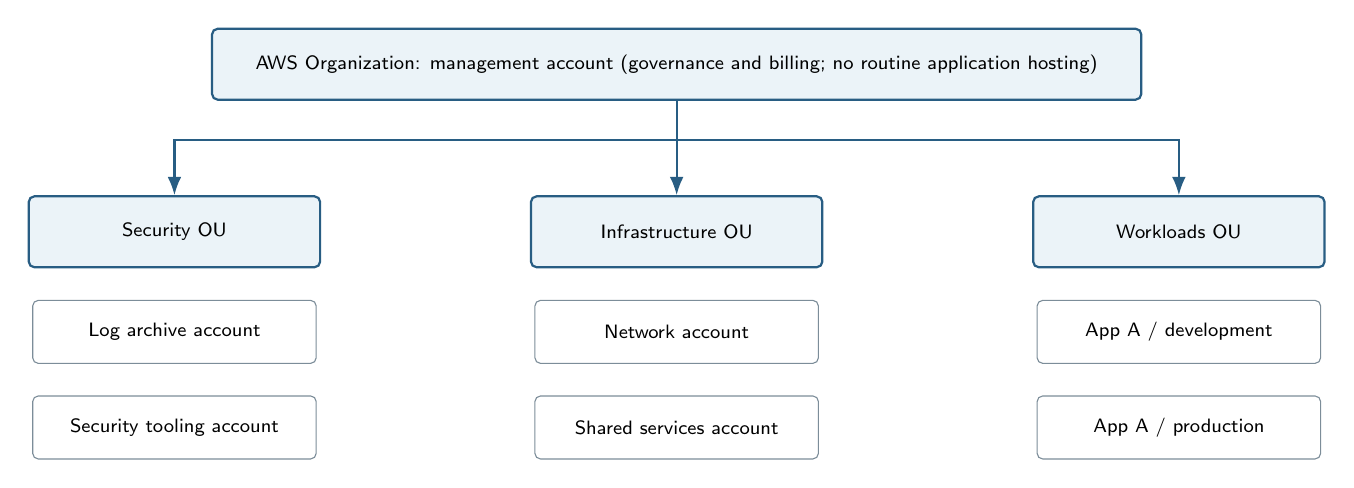
\begin{tikzpicture}[
  font=\sffamily\scriptsize,
  node distance=5mm,
  base/.style={draw=MidBlue,thick,rounded corners=2pt,align=center,minimum height=9mm,inner sep=4pt,fill=SoftBlue},
  ou/.style={base,minimum width=37mm},
  acct/.style={draw=MidGray,rounded corners=2pt,align=center,inner sep=3pt,fill=white,minimum height=8mm,minimum width=36mm},
  line/.style={-Latex,thick,draw=MidBlue}]
\node[base,minimum width=118mm] (org) {AWS Organization: management account (governance and billing; no routine application hosting)};
\node[ou,below left=12mm and -14mm of org] (sec) {Security OU};
\node[ou,below=12mm of org] (infra) {Infrastructure OU};
\node[ou,below right=12mm and -14mm of org] (work) {Workloads OU};
\node[acct,below=4mm of sec] (logs) {Log archive account};
\node[acct,below=4mm of logs] (audit) {Security tooling account};
\node[acct,below=4mm of infra] (net) {Network account};
\node[acct,below=4mm of net] (shared) {Shared services account};
\node[acct,below=4mm of work] (dev) {App A / development};
\node[acct,below=4mm of dev] (prod) {App A / production};
\draw[line] (org.south) -- ++(0,-5mm) -| (sec.north);
\draw[line] (org.south) -- (infra.north);
\draw[line] (org.south) -- ++(0,-5mm) -| (work.north);
\end{tikzpicture}
}\caption{Illustrative AWS Organization and account decomposition. The test environment may occupy an additional workload account.}\end{figure}
\subsection{Account placement policy}
\begin{enumerate}
\item \must\ place production and nonproduction in separate AWS accounts for applications covered by this baseline. Where risk warrants, isolate each critical workload or data-sensitivity domain in separate accounts.
\item \must\ separate security logging and monitoring administration from ordinary application deployment; prevent routine workload principals from modifying organization-wide audit evidence.
\item \must\ apply OU-level SCP guardrails where supported. SCPs restrict the maximum permission set and do not grant permissions.
\item \must\ define account ownership, allowed AWS Regions, permitted network egress patterns, tagging, backup, and incident contacts before onboarding an application.
\item \should\ use a centrally governed account-vending process rather than creating accounts ad hoc from application workflows.
\end{enumerate}
\subsection{Deployment roles and environment mapping}
A deployment role is scoped to one \emph{application + environment + AWS account} combination. State backends are at minimum per account and environment, with unique object keys and narrowly scoped permissions. Even if two nonproduction environments share an AWS account under an approved exception, they retain separate state keys and independent IAM roles; that does not constitute the same isolation assurance as separate accounts.

\section{Explicit trust boundaries}
\subsection{Identity and state boundaries}
\begin{figure}[htbp]\centering\resizebox{0.92\linewidth}{!}{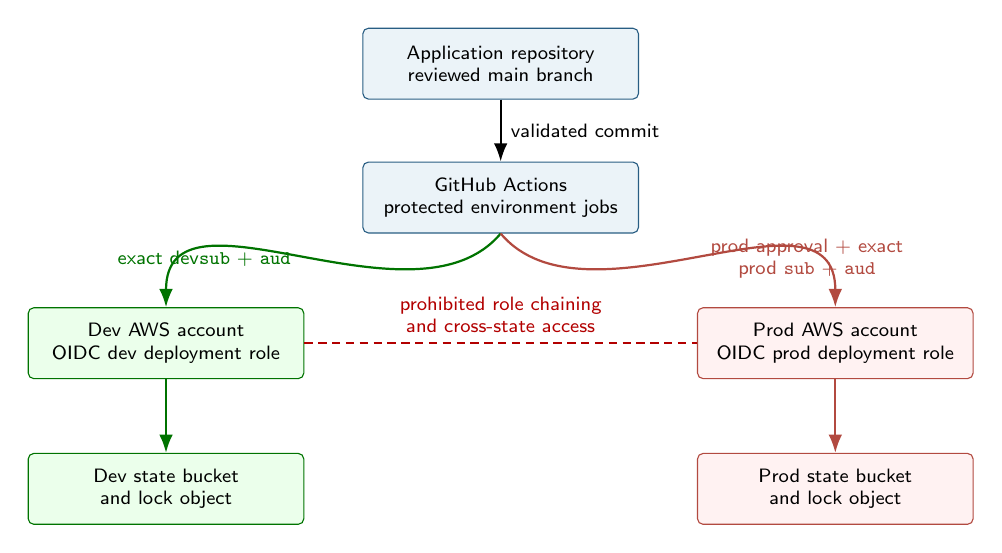
\begin{tikzpicture}[font=\sffamily\scriptsize,
  box/.style={draw=MidBlue,rounded corners=2pt,minimum height=9mm,minimum width=35mm,align=center,fill=SoftBlue,inner sep=3pt},
  dev/.style={box,draw=green!45!black,fill=green!8},
  prod/.style={box,draw=Brick,fill=red!5},
  arrow/.style={-Latex,thick},
  blocked/.style={red!70!black,thick,densely dashed}]
\node[box] (repo) at (0,0) {Application repository\\reviewed main branch};
\node[box] (gh) at (0,-1.7) {GitHub Actions\\protected environment jobs};
\node[dev] (drole) at (-4.25,-3.55) {Dev AWS account\\OIDC dev deployment role};
\node[prod] (prole) at (4.25,-3.55) {Prod AWS account\\OIDC prod deployment role};
\node[dev] (dstate) at (-4.25,-5.4) {Dev state bucket\\and lock object};
\node[prod] (pstate) at (4.25,-5.4) {Prod state bucket\\and lock object};
\draw[arrow] (repo) -- node[right]{validated commit} (gh);
\draw[arrow,green!45!black] (gh.south) to[out=230,in=90] node[left,align=center]{exact dev\texttt{sub} + \texttt{aud}} (drole.north);
\draw[arrow,Brick] (gh.south) to[out=310,in=90] node[right,align=center]{prod approval + exact\\prod \texttt{sub} + \texttt{aud}} (prole.north);
\draw[arrow,green!45!black] (drole) -- (dstate);
\draw[arrow,Brick] (prole) -- (pstate);
\draw[blocked] (drole.east) -- node[above,align=center]{prohibited role chaining\\and cross-state access} (prole.west);
\end{tikzpicture}
}\caption{Deployment identity and state boundaries. The prohibited lateral path represents an explicit authorization requirement, not a claim that network routing alone prevents privilege escalation.}\end{figure}
\subsection{GitHub OIDC authorization}
The AWS IAM provider for GitHub Actions uses \texttt{https://token.actions.githubusercontent.com} and an audience of \texttt{sts.amazonaws.com} in the commercial AWS partition. Each role's trust policy \must\ use \texttt{StringEquals} for both \texttt{aud} and the full expected \texttt{sub}. An environment-scoped workflow normally produces a subject ending in \texttt{:environment:prod}; this subject does \emph{not} simultaneously encode a branch reference. Therefore a protected GitHub environment must separately restrict deployment branches and reviewer authority.

GitHub introduced immutable owner/repository identifiers in default subject formats for eligible new/renamed repositories beginning 15 July 2026. The exact token format varies by repository, host, environment, and opt-in state. \must\ inspect the actual subject before constructing trust. Never guess ID numbers or replace a strict subject with a wide wildcard merely to make authentication succeed. See \S\ref{sec:refs}.
\begin{minted}[fontsize=\scriptsize,breaklines,frame=lines]{text}
# Illustrative only; provision with the OIDC role example and real values:
"Condition": {"StringEquals": {
  "token.actions.githubusercontent.com:aud": "sts.amazonaws.com",
  "token.actions.githubusercontent.com:sub":
    "repo:ORG@OWNER_ID/REPO@REPO_ID:environment:prod"
}}
\end{minted}
\subsection{Trust-boundary verification tests}
\begin{enumerate}
\item A production workflow with the approved repo/environment token \emph{can} assume only the prod role.
\item A development environment token, pull-request job, unrelated repo token, and incorrect audience \emph{cannot} assume the prod role.
\item The dev role \emph{cannot} use \texttt{sts:AssumeRole} to enter prod, mutate prod state, or disable centralized logging.
\item Every deploy checks actual caller account ID against the expected environment account before \texttt{terraform init}.
\end{enumerate}

\section{Terraform module and state governance}
\subsection{Module contract}
A reusable module \must\ include an owner, version, supported Terraform/provider constraints, inputs/outputs, security defaults, examples, a changelog, tests, and an explicit compatibility policy. Modules \must\ not embed access keys or create unbounded administrator policies. Consumption \must\ be pinned to immutable releases or commit references; production promotion is a reviewed change.
\subsection{Root modules, backends, and separation}
Each application-environment root \must\ have an independent state path and deployment principal. State is a sensitive artifact, regardless of \texttt{sensitive = true}; plan files may also contain credentials and protected attributes. S3 backend encryption, bucket versioning, public access blocking, and TLS-only policies are required. \texttt{use\_lockfile = true} is the default locking method for supported Terraform versions; DynamoDB-based locking is deprecated. An S3 lock file needs \texttt{GetObject}, \texttt{PutObject}, and \texttt{DeleteObject} permission \emph{on the lock object only}, not deletion permission on the state object itself.
\begin{minted}[fontsize=\scriptsize,breaklines,frame=lines]{text}
terraform {
  backend "s3" {
    key          = "applications/sample-app/prod/terraform.tfstate"
    encrypt      = true
    use_lockfile = true
    # bucket and region are configured at init (not secrets)
  }
}
\end{minted}
\subsection{State bootstrap is separately privileged}
State buckets, identity providers, and deployment roles form the \emph{bootstrap layer}. Application deployment roles cannot safely create or administer their own privilege boundaries. Bootstrap changes require separate platform owner reviews, isolated bootstrap state, break-glass documentation, and audited privileged execution. Recovery must cover deleted state objects, lost lock files, unauthorized backend changes, and compromised deployment roles. Lock-file removal is a controlled operational procedure; never use \texttt{-lock=false} as a normal pipeline workaround.
\subsection{Cross-state coupling}
Avoid unrestricted \texttt{terraform\_remote\_state} access. Share narrow nonsecret interface values via controlled service discovery, approved parameter services, or explicitly scoped outputs. A consumer role must not be granted broad access to a producer's entire state merely to read one endpoint.

\section{CI/CD and release governance}
\subsection{Required promotion model}
\begin{figure}[htbp]\centering\resizebox{0.98\linewidth}{!}{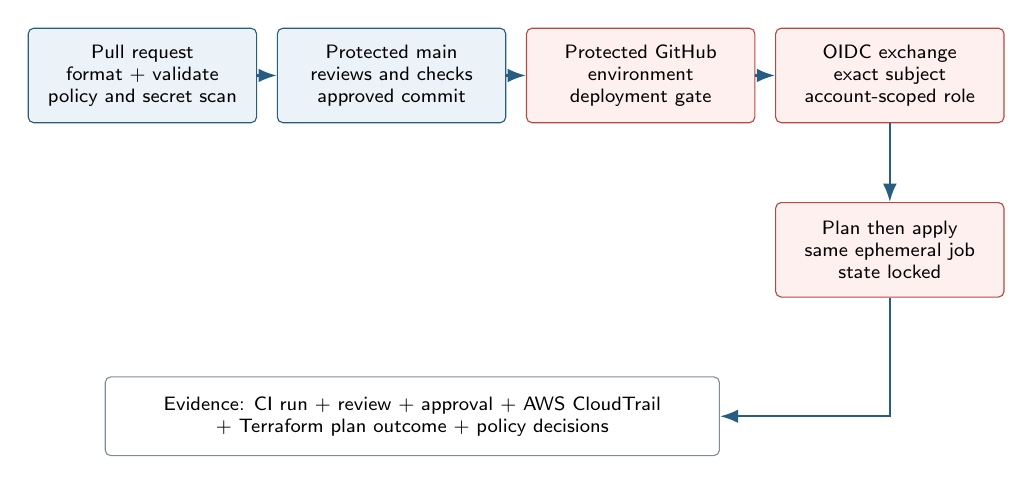
\begin{tikzpicture}[font=\sffamily\scriptsize,node distance=2.5mm,
 phase/.style={draw=MidBlue,rounded corners=2pt,minimum width=29mm,minimum height=12mm,align=center,fill=SoftBlue,inner sep=3pt},
 secure/.style={phase,draw=Brick,fill=red!6},
 arr/.style={-Latex,thick,draw=MidBlue}]
\node[phase] (pr) {Pull request\\format + validate\\policy and secret scan};
\node[phase,right=of pr] (merge) {Protected main\\reviews and checks\\approved commit};
\node[secure,right=of merge] (env) {Protected GitHub\\environment\\deployment gate};
\node[secure,right=of env] (oidc) {OIDC exchange\\exact subject\\account-scoped role};
\node[secure,below=10mm of oidc] (apply) {Plan then apply\\same ephemeral job\\state locked};
\draw[arr] (pr)--(merge);
\draw[arr] (merge)--(env);
\draw[arr] (env)--(oidc);
\draw[arr] (oidc)--(apply);
\node[draw=MidGray,rounded corners=2pt,fill=white,align=center,minimum width=78mm,minimum height=10mm,below left=10mm and 7mm of apply] (evidence) {Evidence: CI run + review + approval + AWS CloudTrail\\ + Terraform plan outcome + policy decisions};
\draw[arr] (apply.south) |- (evidence.east);
\end{tikzpicture}
}\caption{Predeployment and production deployment evidence chain.}\end{figure}
\begin{enumerate}
\item Untrusted pull requests \must\ run static validation and scans \emph{without} AWS deploy credentials or OIDC token permission.
\item GitHub rulesets \must\ require approved reviews, successful checks, and protection of workflow/IaC changes before merging to the deployment branch.
\item Production deployment \must\ use a protected GitHub environment and a distinct AWS role. If GitHub plan restrictions prevent an adequate independent approval gate, an approved external deployment-approval system \must\ substitute; do not assume the feature exists.
\item Deploy jobs \must\ select the account, state key, and environment from protected configuration; verify AWS caller identity and prevent deployments from unapproved branch/event contexts.
\item Terraform \must\ lock state; plan and apply \should\ be performed against the same approved revision and exact saved plan. Saved plans must not be publicly uploaded.
\item All third-party actions \must\ use organization-approved immutable references or supported workflow dependency lockfiles. Supply-chain scanning, secret detection, Terraform policy checks, and provider lockfiles \must\ be enforced as required checks.
\end{enumerate}
\subsection{High-assurance production deployments}
For regulated/high-criticality workloads, use an independent change approval, signed build provenance, reusable workflows maintained in a restricted repository, artifact attestations, short-lived runner isolation, and explicit two-person authorization. GitHub built-in required-reviewer semantics and availability depend on plan and configuration and do not automatically establish dual independent approval.
\subsection{Pull request and deployment IAM separation}
The CI validation example omits \texttt{id-token: write}. The deployment example grants that permission only on the environment-bound job. Avoid \texttt{pull\_request\_target} for executing untrusted code, and prevent reusable workflows from expanding permission scope. Self-hosted runner compromise is treated as a privileged infrastructure risk requiring ephemeral runners, network separation, and credential cleanup.

\section{Security control matrix}
\small
\setlength{\LTleft}{0pt}\setlength{\LTright}{0pt}
\begin{longtable}{@{}p{13mm}p{39mm}p{64mm}p{34mm}@{}}
\caption{Normative controls; evidence is retained under organization-specific retention policy.}\\
\toprule ID & Control objective & Requirement / validation & Primary evidence\\\midrule\endfirsthead
\toprule ID & Control objective & Requirement / validation & Primary evidence\\\midrule\endhead
\ctrl{REP-01} & Repository ownership & Each root has named owner, codeowners, service inventory & Catalog + CODEOWNERS\\
\ctrl{REP-02} & Protected changes & IaC/workflows require review and passing checks & Ruleset export + PRs\\
\ctrl{REP-03} & Module provenance & Approved source and immutable version/ref & Module inventory + lock files\\
\ctrl{ACC-01} & AWS account separation & Prod and nonprod isolated, target ID checked & Account inventory + STS logs\\
\ctrl{ACC-02} & Organization guardrails & Baseline SCPs and centralized audit controls & OU/SCP + service config\\
\ctrl{ACC-03} & Restricted bootstrap & Privileged bootstrap separate from deploy role & Access review + CloudTrail\\
\ctrl{IAM-01} & Identity federation & No long-lived deployment access keys & IAM/Secrets inventory\\
\ctrl{IAM-02} & OIDC trust & Exact per-repo + environment subject and audience & Role trust policy + negative tests\\
\ctrl{IAM-03} & Deployment least privilege & Resource-scoped role, documented wildcard exceptions & IAM policy simulation\\
\ctrl{IAM-04} & No role lateral movement & Dev identity cannot assume prod or access prod state & Negative auth test\\
\ctrl{STA-01} & State segregation & Unique bucket/account and unique path for each env & Backend inventory\\
\ctrl{STA-02} & State confidentiality & Encryption, TLS-only, no public access & AWS Config or policy audit\\
\ctrl{STA-03} & State integrity/recovery & Versioning, lockfile, tested recovery & S3 config + restore evidence\\
\ctrl{STA-04} & Restrict sensitive artifacts & State/plan access limited, retention controlled & Access logs + pipeline logs\\
\ctrl{CIC-01} & Untrusted PR isolation & PR validation has no cloud deploy credentials & Workflow config + test\\
\ctrl{CIC-02} & Production approval & Independent branch/environment approval enforced & Deployment evidence\\
\ctrl{CIC-03} & Dependency pinning & Actions, Terraform providers, modules approved & Locked dependencies\\
\ctrl{CIC-04} & Deployment correctness & Exact plan, protected workflow, account assertion & Workflow trace + run ID\\
\ctrl{SEC-01} & Policy-as-code & IaC misconfiguration checks block merge & Checkov/Trivy/OPA report\\
\ctrl{SEC-02} & Secret scanning & Commit/PR secret controls; response SLA & Alert history + PR check\\
\ctrl{OPS-01} & Evidence and detection & CloudTrail/Config/GitHub audit centrally preserved & Log archive + alerts\\
\ctrl{OPS-02} & Drift and remediation & Schedule drift scans, owner response SLAs & Drift ticket + disposition\\
\ctrl{OPS-03} & Recovery & State recovery and emergency access exercised & Exercise record\\
\ctrl{GOV-01} & Standards exceptions & Expiration, owner, compensating controls, signoff & Exception register\\\bottomrule
\end{longtable}
\normalsize

\section{Responsibility allocation and evidence}
\begin{center}\small\begin{tabularx}{\linewidth}{@{}p{47mm}p{29mm}p{30mm}X@{}}\toprule
Activity & Accountable & Responsible & Consulted / informed\\\midrule
Account vending / OU guardrails & Cloud governance & Platform & Security / Audit\\
OIDC trust / bootstrap roles & Security Architecture & Platform IAM & App owner / Audit\\
Terraform module release & Platform lead & Module maintainers & Security / App owners\\
Application changes / test evidence & App engineering lead & App engineers & AppSec / SRE\\
Production deploy authorization & Change authority & Release owner & Security / SRE\\
State restoration / IAM incident & Platform on-call & Platform + SecOps & App owner / Audit\\\bottomrule\end{tabularx}\end{center}
Every production deployment record \must\ identify the repository, commit SHA, workflow run ID, actor, approved environment, AWS account ID, IAM role session, policy result, and change ticket if required. Logs \should\ support reconstruction even if the original repository is renamed or archived.

\section{Conformance tests and acceptance criteria}
\begin{enumerate}
\item \textbf{Repository control check:} attempt an unreviewed workflow/IaC change on the protected branch; expected result: blocked.
\item \textbf{Federation negative checks:} exercise wrong repository, wrong environment, wrong audience, dev-to-prod attempt; expected result: STS denies all.
\item \textbf{State negative checks:} dev principal reads prod state and deletes state object; expected result: access denied. Authorized lock-file deletion is limited to the lock key.
\item \textbf{Account binding test:} change expected account ID to a nonmatching value; expected result: deployment stops before Terraform init.
\item \textbf{Supply-chain check:} submit an unapproved action/module release; expected result: required policy gate blocks merge.
\item \textbf{Recovery test:} recover a versioned S3 state snapshot under approved break-glass procedure, verify consistency, and document audit events.
\item \textbf{Audit trace:} select a release and reconstruct approved PR, exact commit, job, STS caller and AWS activity.
\end{enumerate}
Evidence is evaluated per control: \textbf{Pass}, \textbf{Fail}, \textbf{Not applicable (with rationale)}, or \textbf{Exception approved}. Unsupported claims of ''full compliance'' are prohibited.

\section{Migration and implementation roadmap}
\begin{description}[style=nextline,leftmargin=6mm,labelwidth=0pt]
\item[Phase 0---Discovery and classification] Inventory repos, Terraform roots, state keys, identities, GitHub environments, AWS accounts, production data, and shared resources. Identify unmanaged state and long-lived keys.
\item[Phase 1---Platform foundation] Establish AWS Organizations/OUs, log archive, identity management, state buckets, bootstrap roles and approved repo templates; validate SCP impact in nonproduction.
\item[Phase 2---Pilot application] Move a low-risk service to separate dev/prod accounts, exact OIDC trust, scoped backend keys, branch rules, and required checks. Test negative paths and recovery.
\item[Phase 3---Standardization] Publish hardened modules and reusable workflows; require reviewed immutable references; implement central inventory and automated conformance evidence.
\item[Phase 4---Scale and assure] Migrate remaining applications by risk, retire credentials, run drift/incident exercises, monitor exceptions, and review the standard quarterly.
\end{description}

\section{Exception and review procedure}
Exceptions contain a unique identifier, requested departure, affected applications/accounts, threat analysis, compensating controls, reason, sponsor, Security Architecture approval, expiration (normally no longer than 90 days), and remediation milestone. High-severity deviations such as shared production/development IAM trust or unrestricted state access require formal risk acceptance and cannot be treated as routine design preferences. A material AWS/GitHub/Terraform behavior change triggers an out-of-cycle review.

\section{ADR register and decision traceability}
The six standalone ADR source documents shipped in \texttt{adrs/} are normative decision records that govern implementation choices. Superseded ADRs remain in history with links to replacements.
\begin{center}\small\begin{tabularx}{\linewidth}{@{}p{23mm}X p{28mm}@{}}\toprule
ADR & Decision & Status\\\midrule
ADR-0001 & Application-aligned repositories; justified monorepo exception & Proposed\\
ADR-0002 & Multi-account workload/environment isolation & Proposed\\
ADR-0003 & S3-backed state with environment-scoped locking and permissions & Proposed\\
ADR-0004 & Exact GitHub OIDC subject trust with protected environments & Proposed\\
ADR-0005 & Versioned shared modules and controlled promotion & Proposed\\
ADR-0006 & Credential-free PR checks and protected production deployment & Proposed\\\bottomrule
\end{tabularx}\end{center}

\section{Reference implementation excerpts}
The following listings are a \emph{small, demonstrable pattern} for a single CloudWatch log group; they do not create a production landing zone. Deploy role bootstrap, environment configuration, organization policy and action SHA verification require platform review. Full source is in \texttt{examples/}.
\subsection{State bucket bootstrap: controls}
\noindent\textbf{State bucket security baseline (bootstrap main.tf)}\par
\inputminted[fontsize=\scriptsize,breaklines,frame=lines]{text}{../examples/terraform/state-bootstrap/main.tf}
\subsection{OIDC trust and narrowly scoped permissions}
\noindent\textbf{Environment-scoped deployment IAM role (main.tf)}\par
\inputminted[fontsize=\scriptsize,breaklines,frame=lines]{text}{../examples/terraform/oidc-deployment-role/main.tf}
\subsection{GitHub pull request validation}
\noindent\textbf{Validation without AWS deployment credentials}\par
\inputminted[fontsize=\scriptsize,breaklines,frame=lines]{text}{../examples/github/workflows/terraform-validate.yml}
\subsection{GitHub protected deployment}
\noindent\textbf{Environment-scoped deployment workflow}\par
\inputminted[fontsize=\scriptsize,breaklines,frame=lines]{text}{../examples/github/workflows/terraform-deploy.yml}

\section{Source register and currency caveats}\label{sec:refs}
Sources were reviewed on 29 October 2026. Normative requirements in this document are the organization's proposed architecture choices, not quotations from these references. Validate provider/action release compatibility and GitHub plan entitlements at adoption time.
\begin{enumerate}
\item AWS Security Reference Architecture, multi-account strategy: \url{https://docs.aws.amazon.com/prescriptive-guidance/latest/security-reference-architecture/introduction.html}
\item AWS SRA account structure: \url{https://docs.aws.amazon.com/prescriptive-guidance/latest/security-reference-architecture/account-structure.html}
\item AWS Well-Architected, separate workloads using accounts: \url{https://docs.aws.amazon.com/wellarchitected/latest/framework/sec_securely_operate_multi_accounts.html}
\item Terraform S3 backend, lockfile and permissions: \url{https://developer.hashicorp.com/terraform/language/backend/s3}
\item Terraform handling of sensitive values and state: \url{https://developer.hashicorp.com/terraform/language/manage-sensitive-data}
\item GitHub OIDC reference and immutable subject claims: \url{https://docs.github.com/en/actions/reference/security/oidc}
\item GitHub: Configuring OIDC in AWS: \url{https://docs.github.com/en/actions/how-tos/secure-your-work/security-harden-deployments/oidc-in-aws}
\item GitHub deployment environment protections and plan restrictions: \url{https://docs.github.com/en/actions/reference/workflows-and-actions/deployments-and-environments}
\item GitHub secure-use guidance (actions pinning): \url{https://docs.github.com/en/actions/reference/security/secure-use}
\item AWS configure-credentials action (subject formats): \url{https://github.com/aws-actions/configure-aws-credentials}
\end{enumerate}

\end{document}
